\documentclass[a4paper]{ctexart}
\usepackage[utf8]{inputenc}
\usepackage[a4paper]{geometry}
\usepackage{graphicx}
\usepackage{hyperref}
\usepackage[heading = false]{ctex}
\usepackage{xcolor}
\usepackage{fontspec}
\usepackage{listings}
\pagestyle{plain}
\geometry{top=1.0cm, bottom=2.0cm}
\lstset{
    basicstyle = \ttfamily,
    commentstyle = \itshape,
    numbers = left,
    numberstyle = \zihao{-5}\ttfamily,
    frame = lrtb
}

\begin{document}
  \begin{titlepage}
      \songti
      \begin{center}
        \vspace*{2cm}
        
\includegraphics[width=0.7\textwidth]{../HDU.png}\\
        \vspace*{1cm}
        {\fontsize{36pt}{0}
          \textbf{机器学习实验\\报\quad 告\\}
        }
        \vspace*{12cm}
        {\fontsize{18pt}{0}
          \makebox[80pt]{\textbf{实验名称}} \underline{\makebox[250pt]{\Large 监督学习之线性回归}}\\
          \vspace*{0.5cm}
          \makebox[80pt]{\textbf{学\qquad 院}} \underline{\makebox[250pt]{\Large 通信工程学院}}\\
          \vspace*{0.5cm}
          \makebox[80pt]{\textbf{专\qquad 业}} \underline{\makebox[250pt]{\Large xxxx}}\\
          \vspace*{0.5cm}
          \makebox[80pt]{\textbf{学\qquad 号}} \underline{\makebox[250pt]{\Large xxxx}}\\
          \vspace*{0.5cm}
          \makebox[80pt]{\textbf{学生姓名}} \underline{\makebox[250pt]{\Large xxx}}\\
        }
      \end{center}
  \end{titlepage}

  \CTEXsetup[format={\Large\bfseries}]{section}

  \newpage
  \section{实验目的}
  使用机器学习方法对面积和房价进行线性回归拟合

  \section{实验内容与要求}
  \begin{itemize}
    \item 使用python sklearn包对房价数据建立线性回归模型并进行训练
    \item 对结果进行可视化
  \end{itemize}

  \section{实验程序与结果}
  \subsection{程序代码}
  \lstinputlisting[language=Python]{lab1.py}
  \subsection{运行结果}
  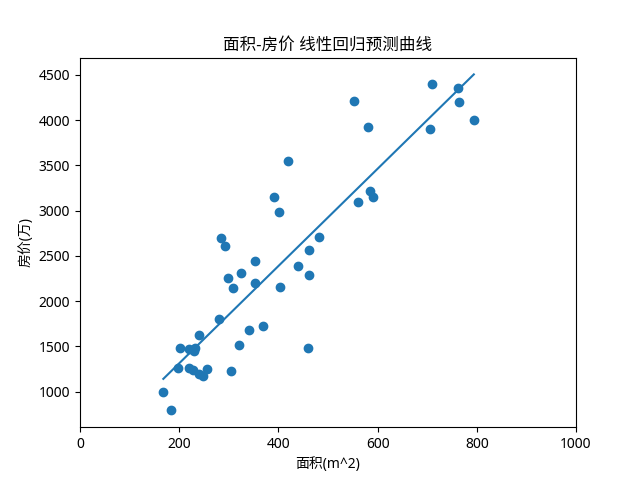
\includegraphics[width=0.7\textwidth]{fig/LR.png}


  \section{实验结果分析}
  从图中可以看出,程序使用线性回归对面积-房价的数据进行预测,得到了一条近似的预测直线

  \section{实验问题解答与体会}
  使用sklearn可以很方便的对数据建立回归模型,但当数据只有一个特征时需要对数据数组进行reshape操作以适应拟合函数所需要的数据格式

\end{document}
